\section{Análisis del Periodo Orbital} \label{metodologia:analisisperiodo}

Una de las propiedades más importantes presente en la curva de luz de una
binaria eclipsante es su \textbf{periodo orbital}. Partiendo del periodo orbital
es posible presentar los datos observacionales en el espacio fase en vez de
tiempo, el cual nos permite ajustar modelos analíticos para determinar ciertas
propiedades del sistema binario. Dada una curva de luz se puede encontrar el
periodo orbital usando \textbf{periodogramas}: herramientas utilizadas para
generar un espectro de potencias para una serie de tiempo periódica. Para series
de tiempo cuyo muestreo no es uniforme en el tiempo (como es común de
observaciones astronómicas) se utiliza el periodograma \textbf{Lomb-Scargle},
derivado de la transformada de Fourier \brakcite{understandingLombScargle}.
Usando un mallado suficientemente fino para explorar el espacio de frecuencias
se puede encontrar la frecuencia de mayor potencia, indicando el periodo orbital
del sistema; al mismo tiempo, para restringir esta malla de periodos se impuso
un límite máximo de 1 día, basado en las primeras observaciones de Iturbide. El
espectro de frecuencias se encuentra en la \reffigure{periodogramaLSFrecs}. 

\begin{figure}[!h]
	\centering
	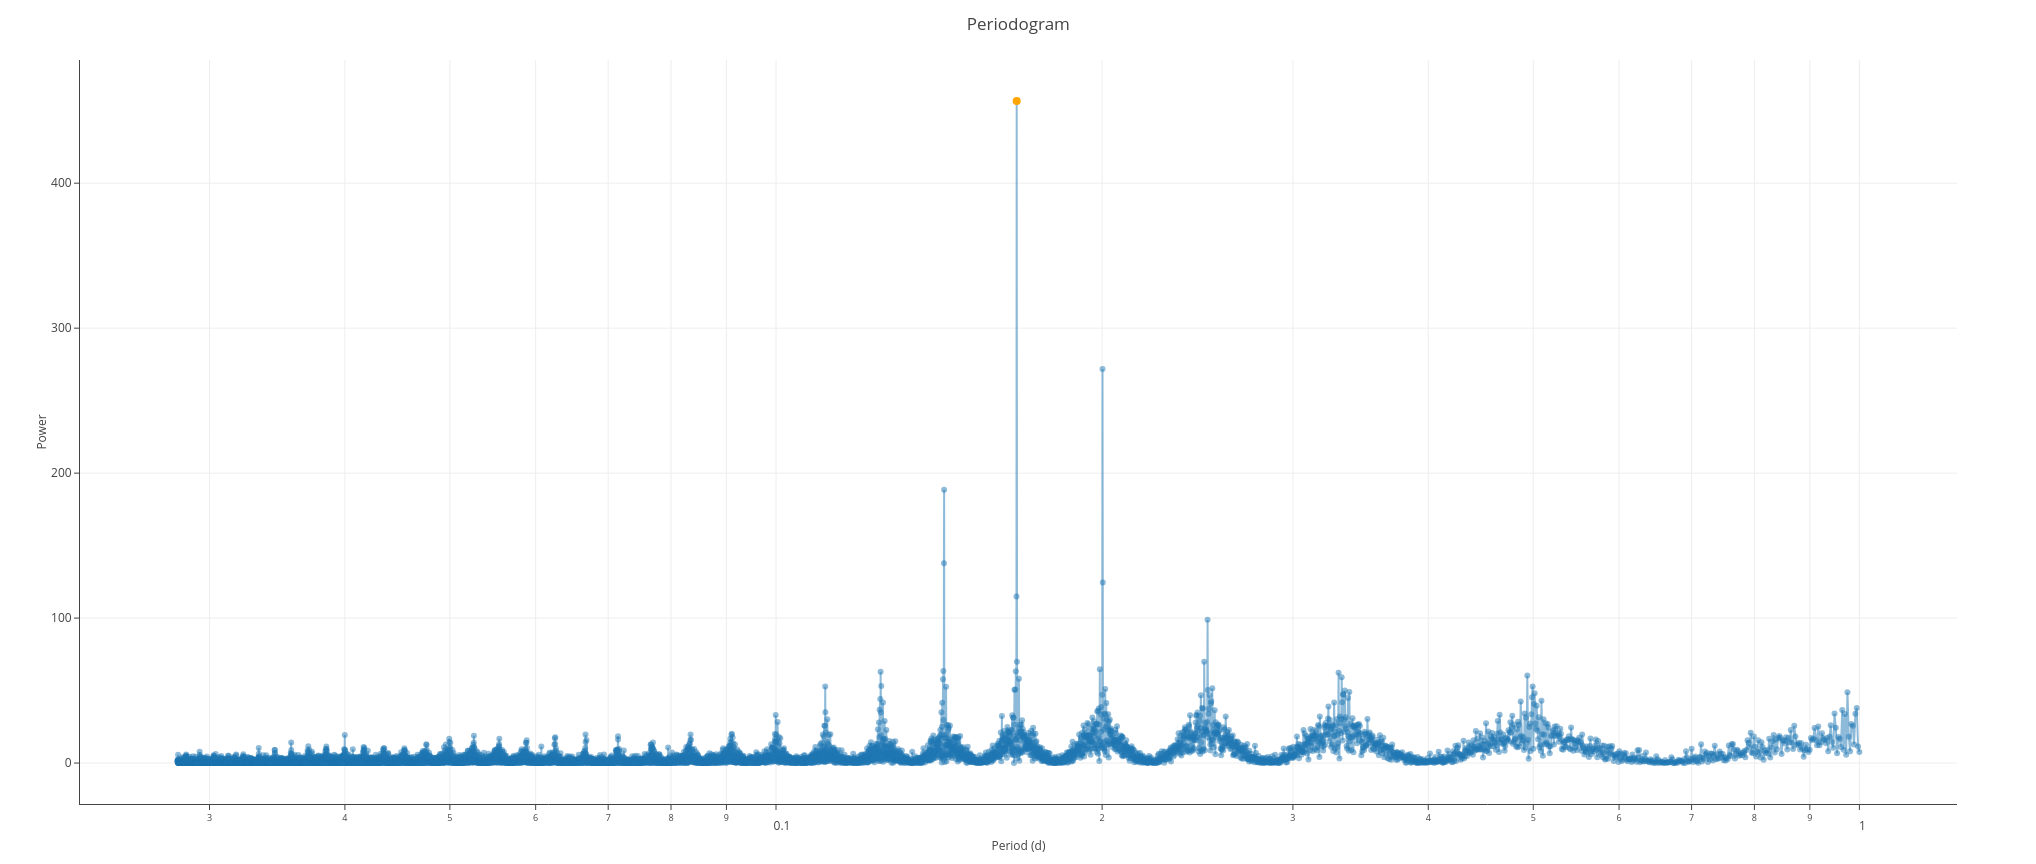
\includegraphics[scale=0.23]{Metodologia/Secciones/AnalisisPeriodo/Figures/IRSA Periodogram.png}
	
	\caption{Espectro de frecuencias de las curvas de luz fotométricas de
	\atoObjIdNoSpace, utilizando observaciones de ZTO en el filtro R. Este
	periodograma fue generado utilizando la herramienta del IRSA dedicada al
	análisis de series de tiempo, \textbf{Time Series Tool}. El pico de más alta
	potencia está ubicado en el periodo de 0.1667834993 d [4.002803983 h]} 
	\label{periodogramaLSFrecs}
\end{figure}

Dado este espectro de frecuencias encontramos que el periodo orbital yace en la
segunda armónica de la frecuencia principal. Esto se debe a los requisitos para
analizar una curva de luz de un sistema binario eclipsante; estos muestran dos
valles en el espacio fase, las cuales corresponden a las etapas en la curva de
luz en las que se observan eclipses en el sistema. Esto es necesario para poder
modelar la curva de luz en fase como una Gaussiana doble, el modelo aceptado
para una binaria eclipsante. %TODO: agrega bibliografía
Utilizando la segunda armónica de la frecuencia de más alta potencia se puede
ver esta forma esperada de la curva de luz, como se puede ver en la
\reffigure{gaiaIturbideZtfPhaseFold}. El periodo orbital encontrado es de
8.005607976 horas.

\begin{figure}[!h]
	\centering
	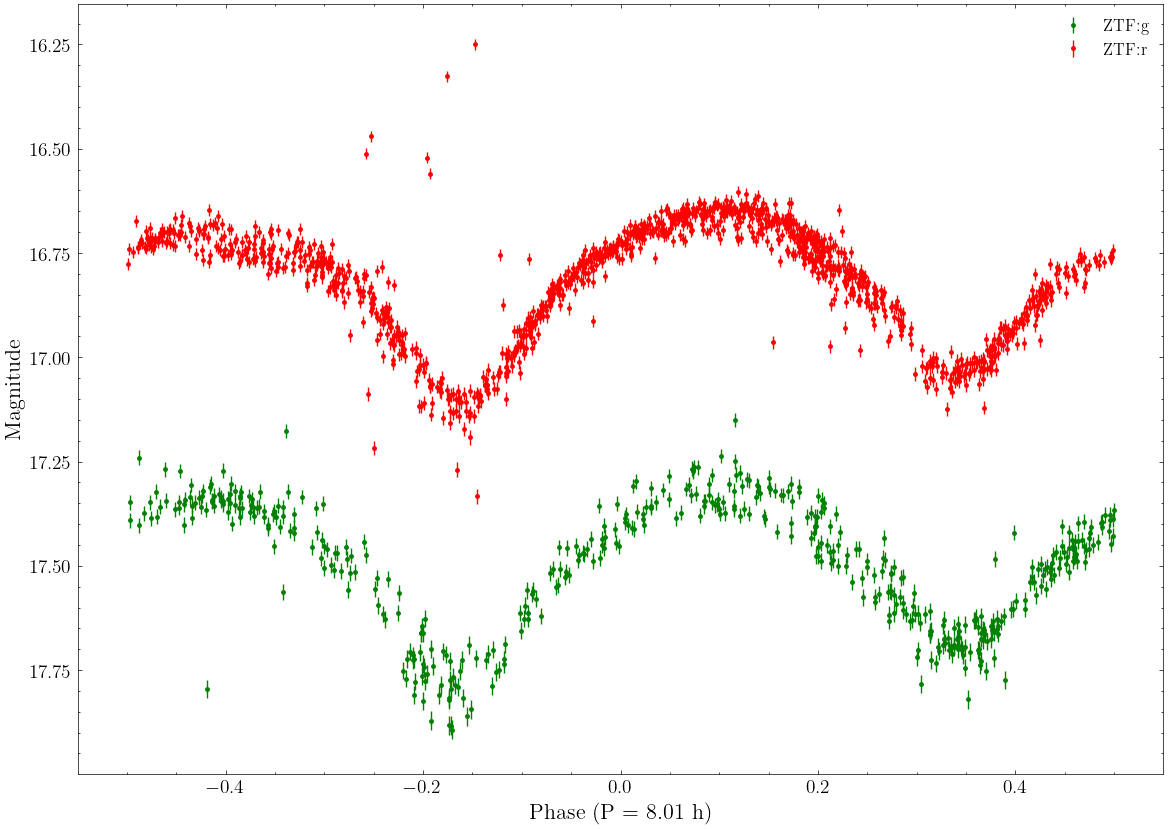
\includegraphics[scale=0.3]{Metodologia/Secciones/AnalisisPeriodo/Figures/ZTF Phase-Folded.png}
	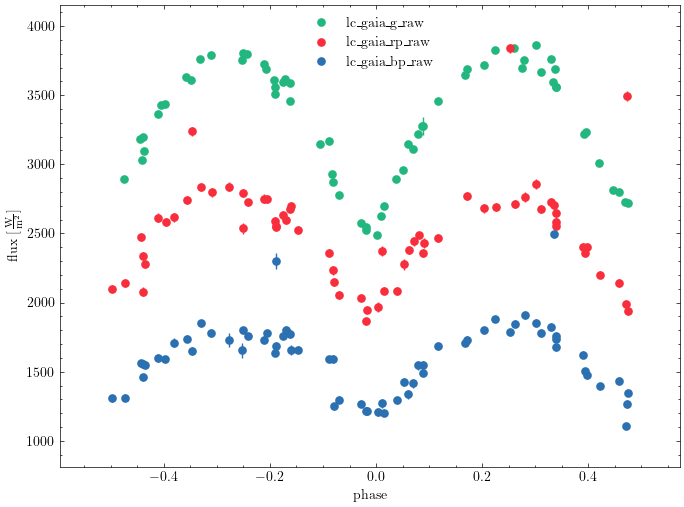
\includegraphics[scale=0.3]{Metodologia/Secciones/AnalisisPeriodo/Figures/Gaia Phase-Folded.png}
	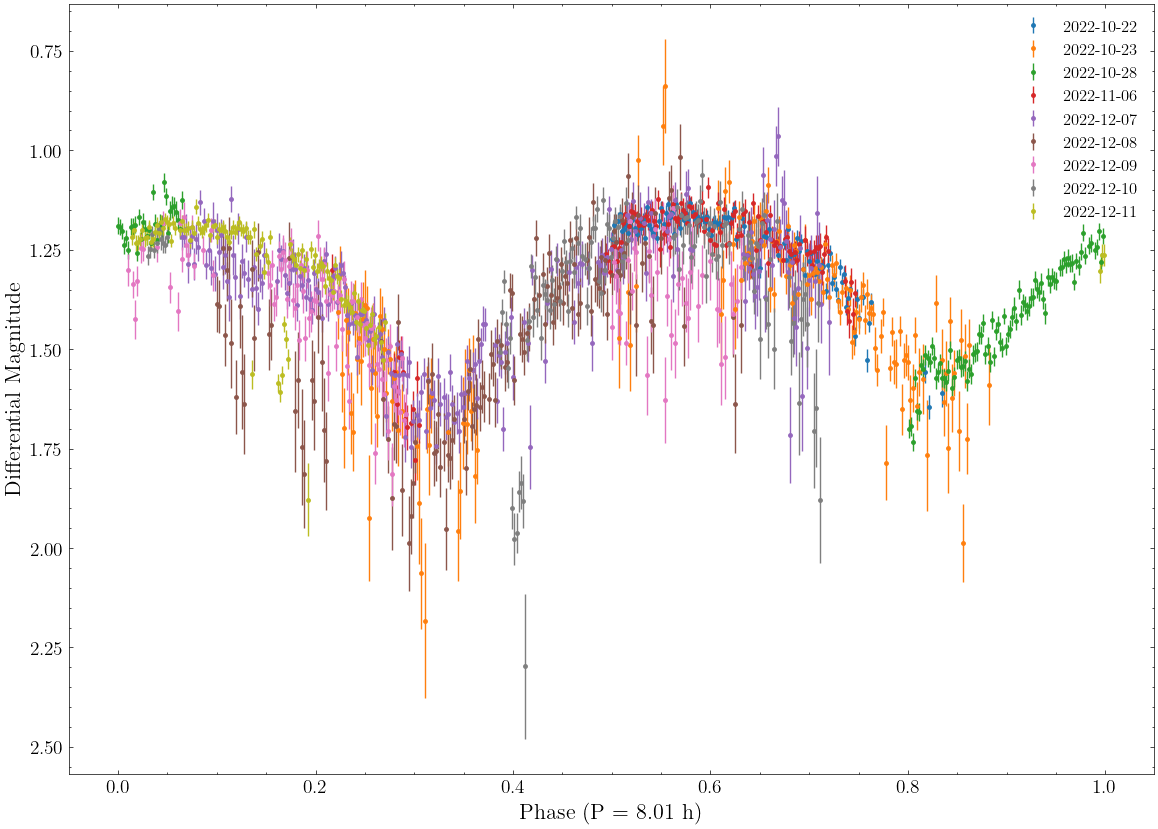
\includegraphics[scale=0.4]{Metodologia/Secciones/AnalisisPeriodo/Figures/Iturbide Phase-Folded.png}

	\caption{Curvas de luz de ZTF, Gaia e Iturbide en espacio fase dado un
		periodo orbital de 8.005607976 horas. El tiempo de conjunción superior
		son corregidos en los siguientes pasos de afinación del modelo de
		PHOEBE, el cual ajusta la fase 0 para que coincidan las 3 curvas de luz.
		Las observaciones de Iturbide se clasifican por su noche de observación,
		indicado por su color.}
	\label{gaiaIturbideZtfPhaseFold}
\end{figure}